\section{Lexikálna analýza}

\subsection{Architektúra skenera}
Lexikálny analyzátor je implementovaný ako deterministický konečný automat, ktorý číta zdrojový kód znak po znaku a na základe aktuálneho stavu a načítaneho znaku prechádza na nové stavy a posiela tokeny.

\subsection{Rozhranie pre parser}
Funkcia \texttt{get\_token(Token *token, Scanner *scanner)} po zavolaní vracia jeden štrukturovaný \texttt{Token} obsahujúci typ tokenu, hodnotu čísla int alebo double alebo dynamicky alokovaný reťazec pre reťazce alebo identifikátory a pozíciu (riadok, stĺpec) pre chybové hlásenia.
\texttt{String\_Buffer} slúži ako interný pracovný buffer skenera a používa sa pri skladaní lexém. 

\subsection{Spracovanie kľúčových slov a identifikátorov}
Identifikátory a kľúčové slová sa najprv načítavajú do bufferu a potom sa pomocou funkcie \texttt{check\_for\_token(const char *identifier)} porovnajú so statickým poľom kľúčových slov jazyka IFJ26 a rozlíšia sa na kľúčové slovo alebo identifikátor.
Ak nájde zhodu, tak pošle token \texttt{TOKEN\_KW\_*}, inak odošle \texttt{TOKEN\_ID\_IDENT} s kópiou názvu identifikátora.

\subsection{Číselné literály}
Automat pri číslach postupne podľa stavu a načítaného znaku rozlíši, či sa jedná o celočíslo, desatinné číslo alebo číslo vo vedeckom zápise.
Znaky \texttt{\_} sa na miestach, kde sa môžu nachádzať, ignorujú (znak \texttt{\_} sa nesmie nachádzať na začiatku alebo na konci čísla a ani za bodkou) a znaky \texttt{e/E} a \texttt{d/D} sa používaju na určenie zápisu čísla.
Pri postupnom čítaní znakov skenerom sa postupne ukladajú do dočasného bufferu \texttt{String\_Buffer} a na konci sa hodnota prevádza pomocou \texttt{strtol()} alebo \texttt{strtod()} s kontrolou pretečenia \texttt{ERANGE / INT\_MAX / INT\_MIN} a neplatných znakov.
Číselné literály sa ukladajú priamo do tokenu do \texttt{int\_value} alebo \texttt{double\_value}.

\subsection{Reťazcové literály}
Automat v jednoriadkovom reťazci kontroluje jednotlivé znaky postupne a ak nájde v reťazci znak \texttt{\textbackslash{}}, tak akceptuje ako ďalší znak iba jeden z piatich povolených, ktoré môžu nasledovať: \texttt{\textbackslash{}\textbackslash{}}, \texttt{\textbackslash{}"}, \texttt{\textbackslash{}n}, \texttt{\textbackslash{}t}, \texttt{\textbackslash{}r}.
Ak sa v reťazci objaví \texttt{EOF} alebo \texttt{LF} alebo sa reťazec neukončí, tak skener vráti chybu \texttt{ERR\_LEXICAL}.
Vo viacriadkovom reťazci kontroluje správny začiatok, koniec a či sa v ňom nenachádza \texttt{EOF}.
Pri reťazcoch sa do tokenu alokuje kópia textu pomocou \texttt{strdup()} do \texttt{string\_value}.

\subsection{Odsadenie}
Skener kontroluje odsadenia pomocou zásobníka \texttt{indent\_stack}, skener si značí, kedy začína nový logický riadok (ignoruje \texttt{LF} v zátvorkách a pri komentároch).
Skener počíta medzery na začiatku logického riadku a porovnáva ich so zásobníkom, vďaka čomu potom posiela tokeny \texttt{TOKEN\_INDENT} a \texttt{TOKEN\_DEDENT}.
Odsadenie smie obsahovať iba medzery, výskyt tabulátora v odsadení logického riadku vedie k lexikálnej chybe \texttt{ERR\_LEXICAL}.

\subsection{Komentáre}
Skener ignoruje riadky s komentármi a podporuje vnorené úrovne viacriadkových komentárov \texttt{/*...*/} pomocou sledovania hĺbky cez premennú \texttt{comment\_depth}.
Ak viacriadkový komentár \texttt{/*...*/} obsahuje znak nového riadku \texttt{\textbackslash n}, tak v tom istom riadku nesmie nasledovať žiadny kód ani výraz, inak dôjde k lexikálnej chybe \texttt{ERR\_LEXICAL}.
Jednoriadkové komentáre sa ukončujú znakmi \texttt{\textbackslash{}n} alebo \texttt{EOF}.
Neukončený viacriadkový komentár spôsobí chybu \texttt{ERR\_LEXICAL}.

\subsection{Reťazcová interpolácia}
Rozšírenie \texttt{INTERPOLATEDS} spracováva jednoriadkové \texttt{s"..."} a viacriadkové \verb|s"""..."""| interpolované reťazce vrátane prázdneho reťazca \verb|s""|.
Automat má stavy pre začiatok interpolácie \texttt{STATE\_S\_ONE/TWO}, pre text, únikové sekvenice a dolár v jednoriadkovom \texttt{STATE\_SINGLE\_TEXT/ESCAPE/ID/DOLLAR} aj viacriadkovom reťazci \texttt{STATE\_MULTI\_TEXT/ID/DOLLAR/ONE/TWO}.
\begin{itemize}
    \item \textbf{Text a začiatok a koniec interpolácie:} Súvislý text sa posiela ako \texttt{TOKEN\_INTERP\_TEXT}.
    Začiatok interpolovaného reťazca sa posiela ako \texttt{TOKEN\_INTERP\_START} a koniec  \texttt{TOKEN\_INTERP\_END}.
    Stav \texttt{STATE\_S} slúži na zistenie, či sa po tomto znaku nachádza interpolovaný reťazec alebo to je kľúčové slovo alebo identifikátor.
    \item \textbf{Posielanie dvoch tokenov:} V prípade že skener potrebuje poslať 2 tokeny naraz tak využíva k tomu \texttt{pending\_interp\_end}, kde si jeden odloží do ďaľšieho volania \texttt{get\_token()}.
    V prípade, že máme prázdny reťazec \verb|s""| alebo pred koncom \verb|s"""..."""| ešte ostal neodoslaný text, tak si to skener uloží do \texttt{pending\_interp\_end} a pri jeho ďaľšom zavolaní túto premennú skontroluje a pošle \texttt{TOKEN\_INTERP\_END}.
    \item \textbf{Interpolácia identifikátoru a výrazu:} Identifikátor produkuje token \texttt{TOKEN\_INTERP\_ID}. \texttt{\$\{výraz\}} ohraničuje vložený výraz tokenmi \texttt{TOKEN\_INTERP\_EXPR\_START} a \texttt{TOKEN\_INTERP\_EXPR\_END}.
    Vnorené zátvorky sú podporované a ich vnútro sa tokenizuje normálnym spôsobom ako mimo interpolovaných reťazcov.
    \item \textbf{Dolár:} \texttt{\$\$} v texte reprezentuje znak \texttt{\$}.
    \item \textbf{Znak nového riadku:} V jednoriadkovej interpolácii znak nového riadku \texttt{\textbackslash{}n} spôsobí chybu \texttt{ERR\_LEXICAL} a nie je povolený.
    Vo viacriadkovej interpolácií je \texttt{\textbackslash{}n} povolený.
\end{itemize}

\subsection{Diagram konečného automatu}
Celkový návrh konečného automatu lexikálneho analyzátora je pre lepšiu čitateľnosť rozdelený na dve časti (obrázky~\ref{fig:diagram_automatu_1} a~\ref{fig:diagram_automatu_2}).

\begin{figure}[htbp]
    \centering
    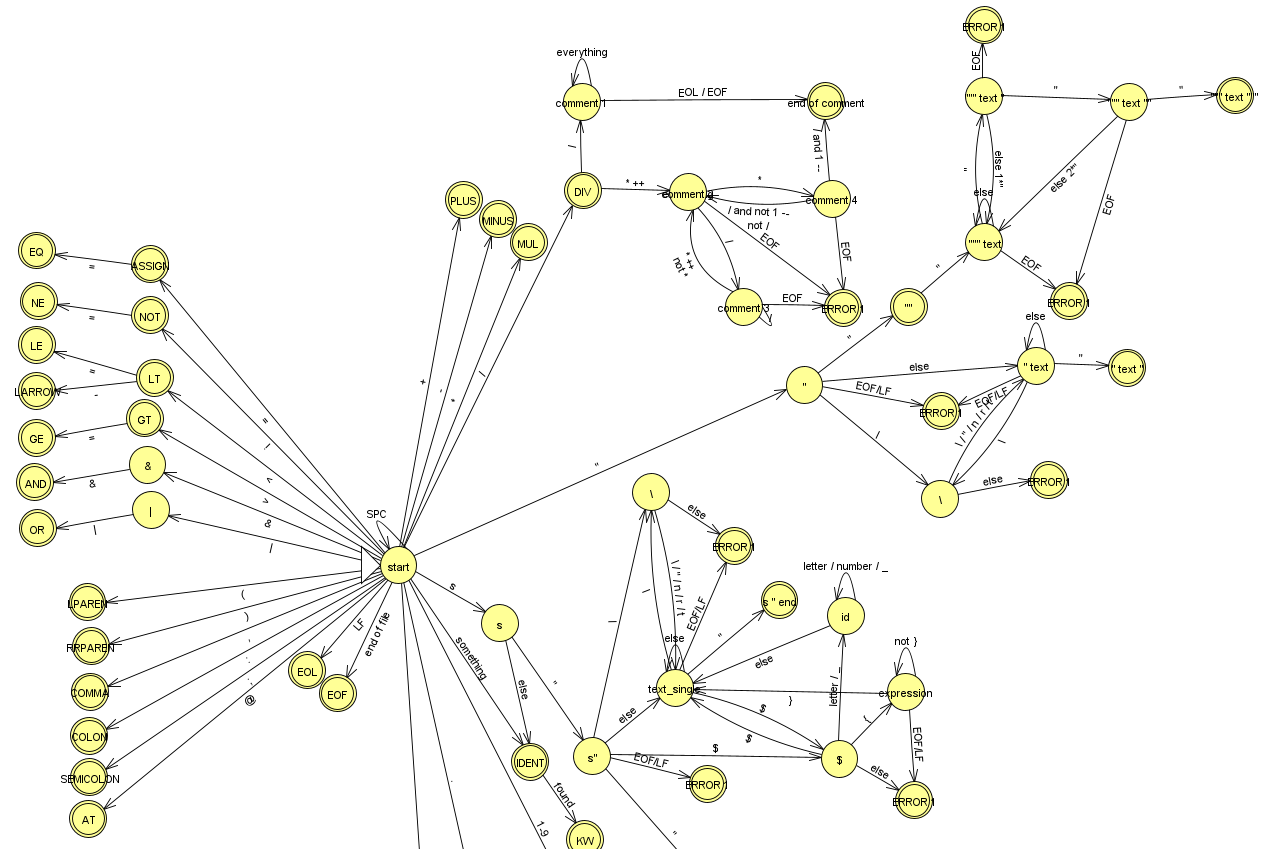
\includegraphics[width=\textwidth,height=0.45\textheight,keepaspectratio]{images/diagram_automatu_1.png}
    \caption{Konečný automat skenera 1. časť (operátory, komentáre, jednoriadkové reťazce a interpolácia)}
    \label{fig:diagram_automatu_1}
\end{figure}

\clearpage

\noindent
\begin{minipage}{\textwidth}
    \centering
    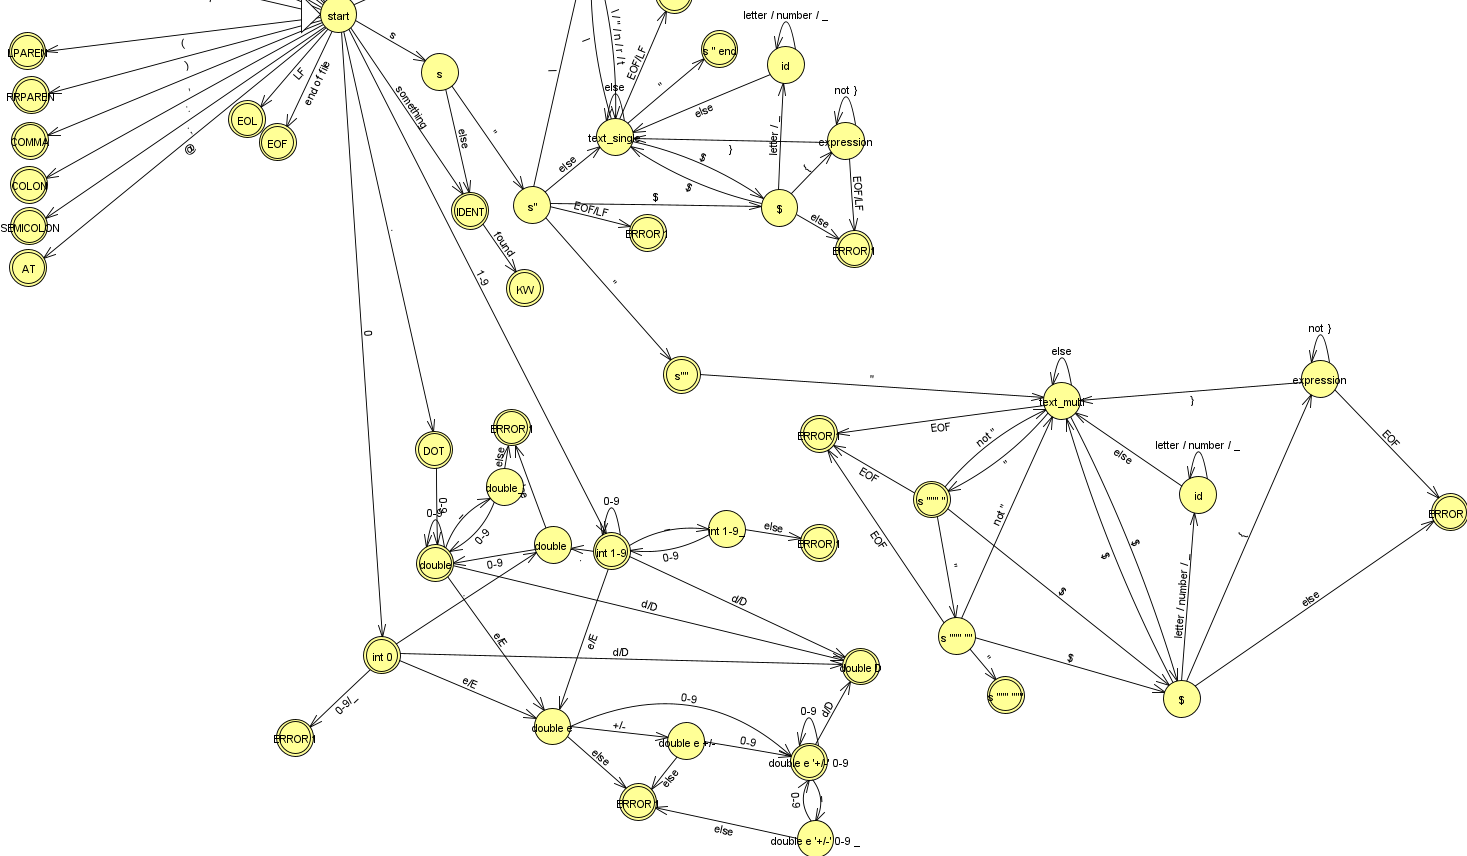
\includegraphics[width=\textwidth,height=0.45\textheight,keepaspectratio]{images/diagram_automatu_2.png}
    \captionof{figure}{Konečný automat skenera 2. časť (číselné literály a viacriadková interpolácia)}
    \label{fig:diagram_automatu_2}
\end{minipage}
\vspace{1em}
